\begin{frame}
\frametitle{Regression of SHAP subgroups vs. hospital thrombolysis}

\begin{center}
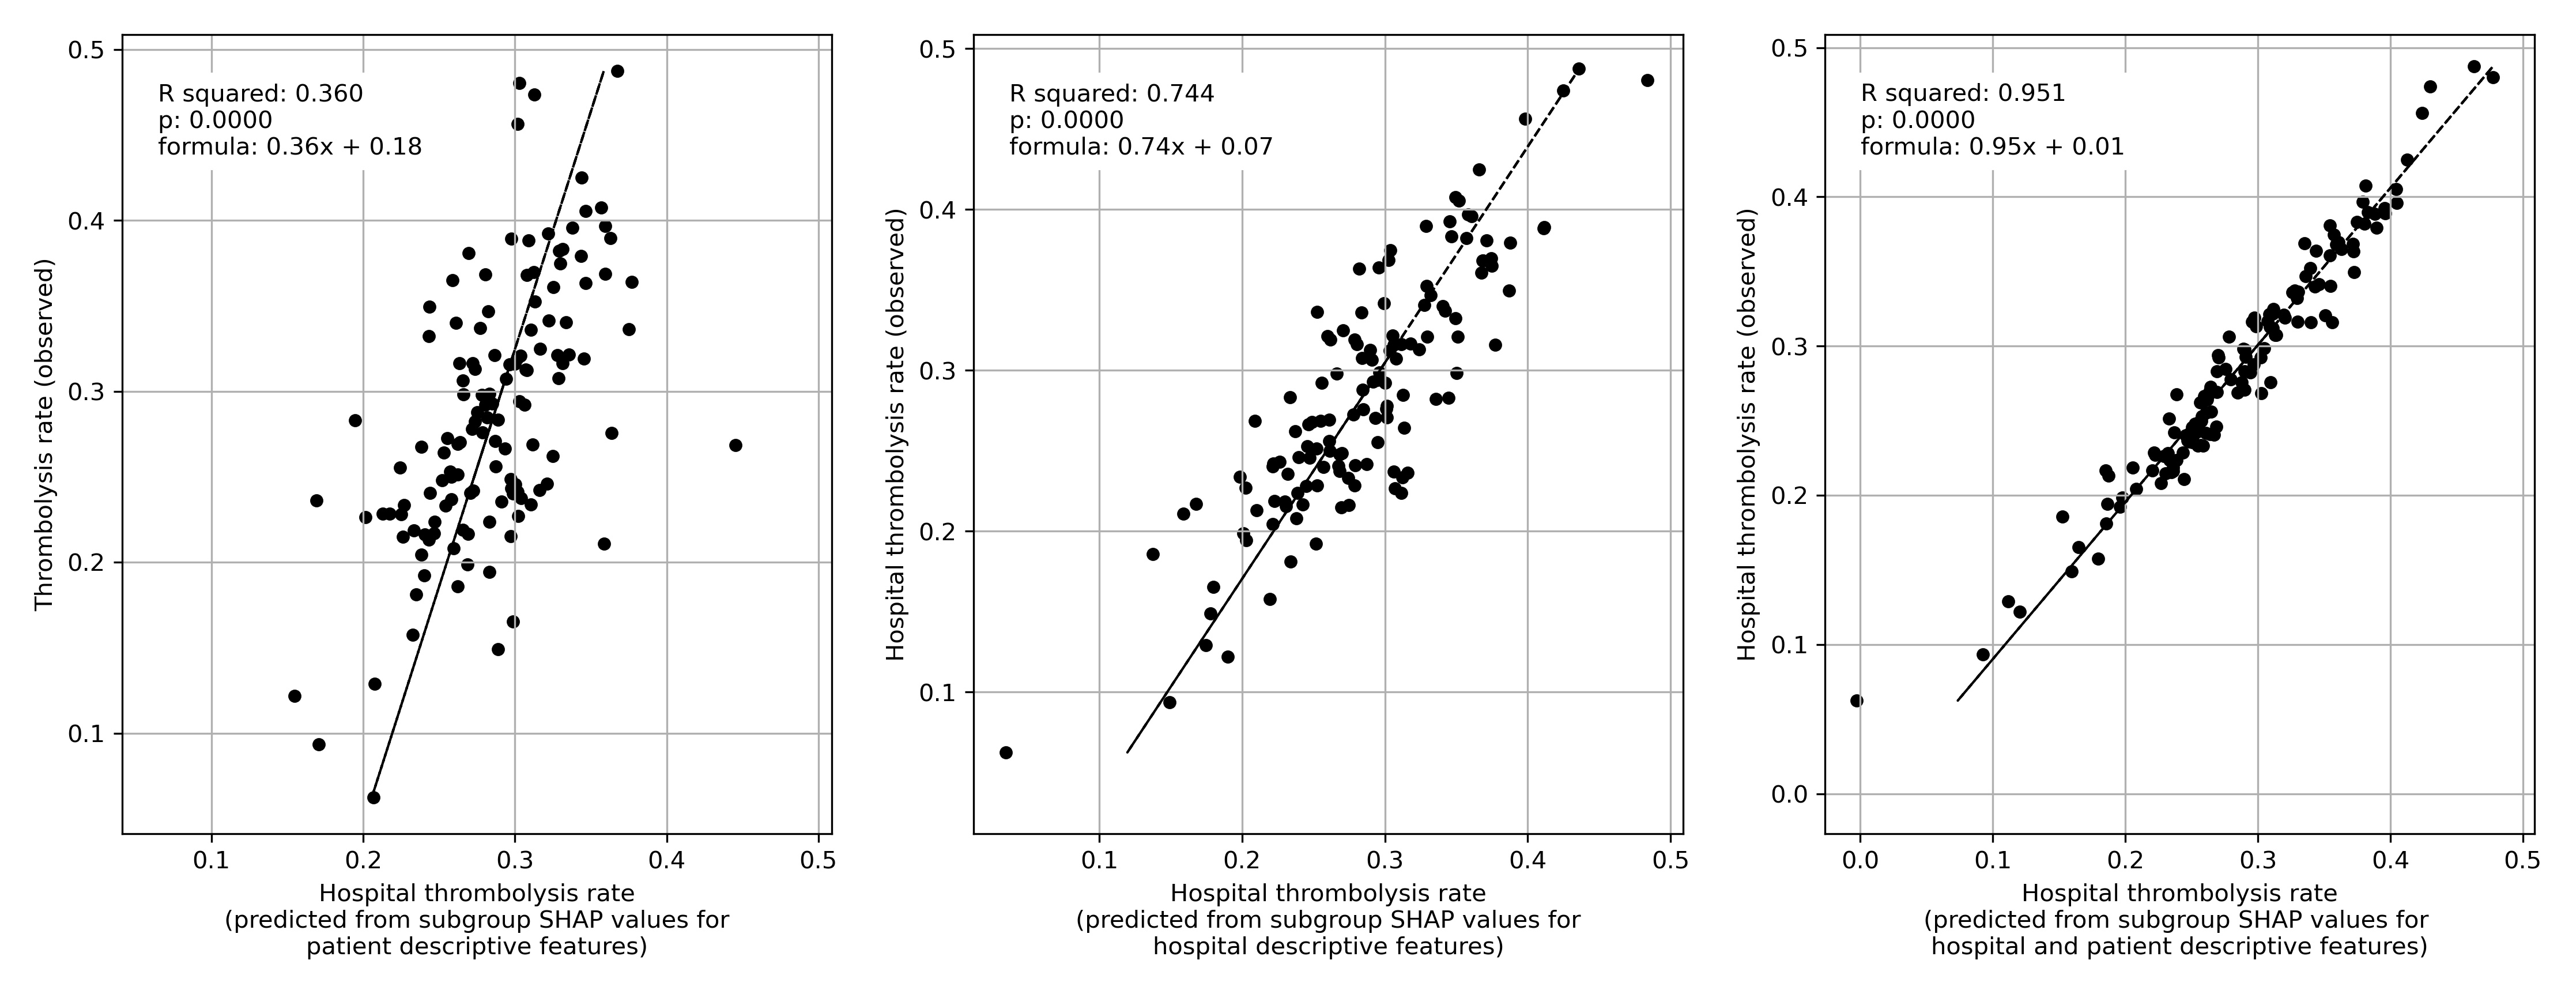
\includegraphics[width=1.0\textwidth]{./images/03e_xgb_10_features_multiple_regression_patient_hosptia_mean.jpg}
\end{center}

\scriptsize
\begin{itemize}
    \item Patient features alone explain 36\% of the variance in hospital thrombolysis use.
    \item Hospital features (hospital ID and arrival-to-scan time) alone explain 74\% of the variance in hospital thrombolysis use.
    \item Together, patient and hospital features explain 95\% of the variance in hospital thrombolysis use.
    \item Note: The sum of the patient-alone and hospital-one features = 110\%, suggesting we have a small amount of shared information between those groups.
\end{itemize}
 
\end{frame}